\documentclass[11pt,a4paper]{article}
\usepackage{amsmath,amssymb,amsthm,graphicx,hyperref,booktabs,placeins}
\usepackage[margin=2.3cm]{geometry}
\newtheorem{proposition}{Proposition}
\graphicspath{{../FIGURES/}}

\title{Regular black holes with cold remnants at a 100\,TeV collider:\\
greybody emission, a full uncertainty budget and the discovery reach}
\author{Project Baby Universe --- Genesis Branch\\ \small(draft for external review; not submitted)}
\date{31 October 2026}

\begin{document}
\maketitle

\begin{abstract}
If gravity becomes strong at a few TeV in $D=4+n$ dimensions and its short-distance completion is a quasi-topological curvature tower,
collider black holes are regular, evaporate towards a zero-temperature extremal remnant, and appear as a hard jet recoiling against an
invisible remnant. We simulate production with real parton distributions, Hawking emission with greybody factors computed on the actual
regular metric, Pythia showering, an FCC-hh detector model with pile-up $\mu=1000$, and a profile-likelihood analysis validated against the
ATLAS $139\,\mathrm{fb}^{-1}$ monojet background ($K=1.18$, $10\%$ rms shape residual). For $n=6$ and $M_D=8$\,TeV the $5\sigma$
discovery reach at 100\,TeV with $30\,\mathrm{ab}^{-1}$ is $M_{\rm ext}=33.4^{+0.8}_{-1.1}$\,TeV and the expected $95\%$ CL exclusion is
$35.0^{+1.2}_{-1.0}$\,TeV, with a documented budget of scale, PDF, normalisation, electroweak, emission-model and detector variations.
Near extremality the regular holes emit gauge bosons at only $7\%$ of the blackbody rate. The signal is separated from a GR black hole
with the same threshold by $13$ selected events, a result that does not depend on the emission model. These are exterior observables;
they test the regular-black-hole tower, not any statement about the interior.
\end{abstract}

\section{Model and generator}
Holes form when the trapped mass $M=y_n\sqrt{\hat s}$ (head-on area bound) exceeds the extremal mass
$M_{\rm ext}=a_n M_D\mu_{\rm ext}(c_l)$ of the tower with length scale $l=c_l/M_D$. The production cross-section uses the
NNPDF2.3 LO parton luminosity times the geometric cross-section with the Yoshino--Nambu form factor. Emission is Monte Carlo
Hawking radiation of Standard Model species on the brane until the remnant is reached; the temperature vanishes at $M_{\rm ext}$.

\paragraph{Greybody factors.} The brane metric is $-f\,dt^2+dr^2/f+r^2d\Omega_2$ with the model-U $f(r)=1-r^2\psi(\mu/r^{D-1})$. We solve
the spin-$0$, $\tfrac12$ and $1$ master equations ($V=f[l(l+1)/r^2+f'/r]$, $W^2+W'$ with $W=k\sqrt f/r$, and $f\,l(l+1)/r^2$) with ingoing
conditions at $r_+$. Checks: $\Gamma_0\to4r_+^2\omega^2$ (horizon area), $\sum(2j+1)\Gamma_j\to(\omega b_c)^2$ (geometric optics), and
agreement with an independent Schwarzschild code to $10^{-4}$.
\begin{proposition}[numerical]
For the $D=10$ Hayward tower, the per-degree-of-freedom number flux relative to the geometric blackbody is (spin $0$, $\tfrac12$, $1$)
$=(1.42,1.01,0.07)$ at $\mu=1.05\mu_{\rm ext}$, $(1.29,1.42,0.94)$ at $3\mu_{\rm ext}$ and $(1.26,1.32,1.09)$ at $10\mu_{\rm ext}$
(Tangherlini $n=6$: $1.23,1.19,1.22$). With Standard Model degrees of freedom the luminosity is $0.92$--$1.32$ of the geometric value and
the spin-1 share of quanta falls from $26\%$ to $2\%$ near the remnant.
\end{proposition}

\section{Detector, backgrounds and statistics}
\begin{itemize}
\item \emph{Backgrounds}: $Z(\nu\nu)$+jet, $W(\ell\nu)$+jet, $t\bar t$ and QCD multijets in $p_T$ slices (Pythia 8.317, NNPDF2.3 QCD+QED
LO), with a normalisation $K=1.18$ fitted at 13\,TeV to the ATLAS monojet background.
\item \emph{Detector}: Delphes FCC-hh card parameters (resolutions, acceptance to $|\eta|<6$), a jet-response tail, pile-up $\mu=1000$
with charged-hadron subtraction and a neutral residual.
\item \emph{Selection}: MET $>1$\,TeV, leading jet $p_T>500$\,GeV, lepton and photon veto, $\Delta\phi(\text{jets},\text{MET})>0.4$;
eight MET bins from 1 to beyond 15\,TeV.
\item \emph{Statistics}: binned profile likelihood with log-normal nuisances (process normalisations 15--20\%, signal 30\%, luminosity 2\%,
jet/MET scale 2\%, MC statistics), auxiliary global observables, Asimov significance; toys reproduce the asymptotic median within
$0.1\sigma$.
\end{itemize}

\section{Reach and uncertainty budget}
\begin{table}[h]\centering\small
\begin{tabular}{llrr}\toprule
Group & Variation & $\Delta$ discovery [TeV] & $\Delta$ exclusion [TeV]\\\midrule
Background & $\mu_R=\mu_F\times2$ / $\times0.5$ (smoothed) & $-0.07$ / $-0.08$ & $-0.07$ / $-0.09$\\
 & PDF CTEQ6L1 / NNPDF3.1 & $+0.09$ / $0.00$ & $+0.08$ / $0.00$\\
 & $K\times1.2$ / $\times0.8$ & $-0.16$ / $+0.21$ & $-0.21$ / $+0.26$\\
Signal & $\sigma\times0.7$ / $\times1.3$ & $-0.48$ / $+0.34$ & $-0.54$ / $+0.39$\\
 & luminosity NNPDF3.1 / mirrored & $-0.66$ / $+0.71$ & $-0.83$ / $+0.95$\\
 & greybody emission & $-0.06$ & $-0.19$\\
Detector & response tail $\times10$ & $-0.62$ & $+0.37$\\
 & degraded pile-up suppression & $-0.33$ & $+0.28$\\
 & scale nuisance $5\%$ & $+0.03$ & $-0.04$\\\midrule
\multicolumn{2}{l}{Total (quadrature)} & $+0.82$ / $-1.10$ & $+1.16$ / $-1.03$\\
\multicolumn{2}{l}{\emph{Not in total}: LL electroweak Sudakov estimate} & $+0.81$ & $+0.91$\\
\bottomrule\end{tabular}
\caption{One-at-a-time shifts of the reach (nominal $33.4$ / $35.0$\,TeV).}\end{table}
The reach is robust to background modelling because the signal falls tenfold per $\sim3$\,TeV of $M_{\rm ext}$; the high-$x$ parton
luminosity dominates. Electroweak corrections (tens of percent at TeV $p_T$; Becher--Garcia i Tormo arXiv:1305.4202, K\"uhn et al.\
hep-ph/0507178) only lower the background and are not counted. Raw generator-variation samples give larger shifts ($0$ to $-0.8$\,TeV)
dominated by Monte Carlo fluctuations in the top MET bins: high-statistics tail samples are required for a real analysis.

\begin{figure}[t]\centering
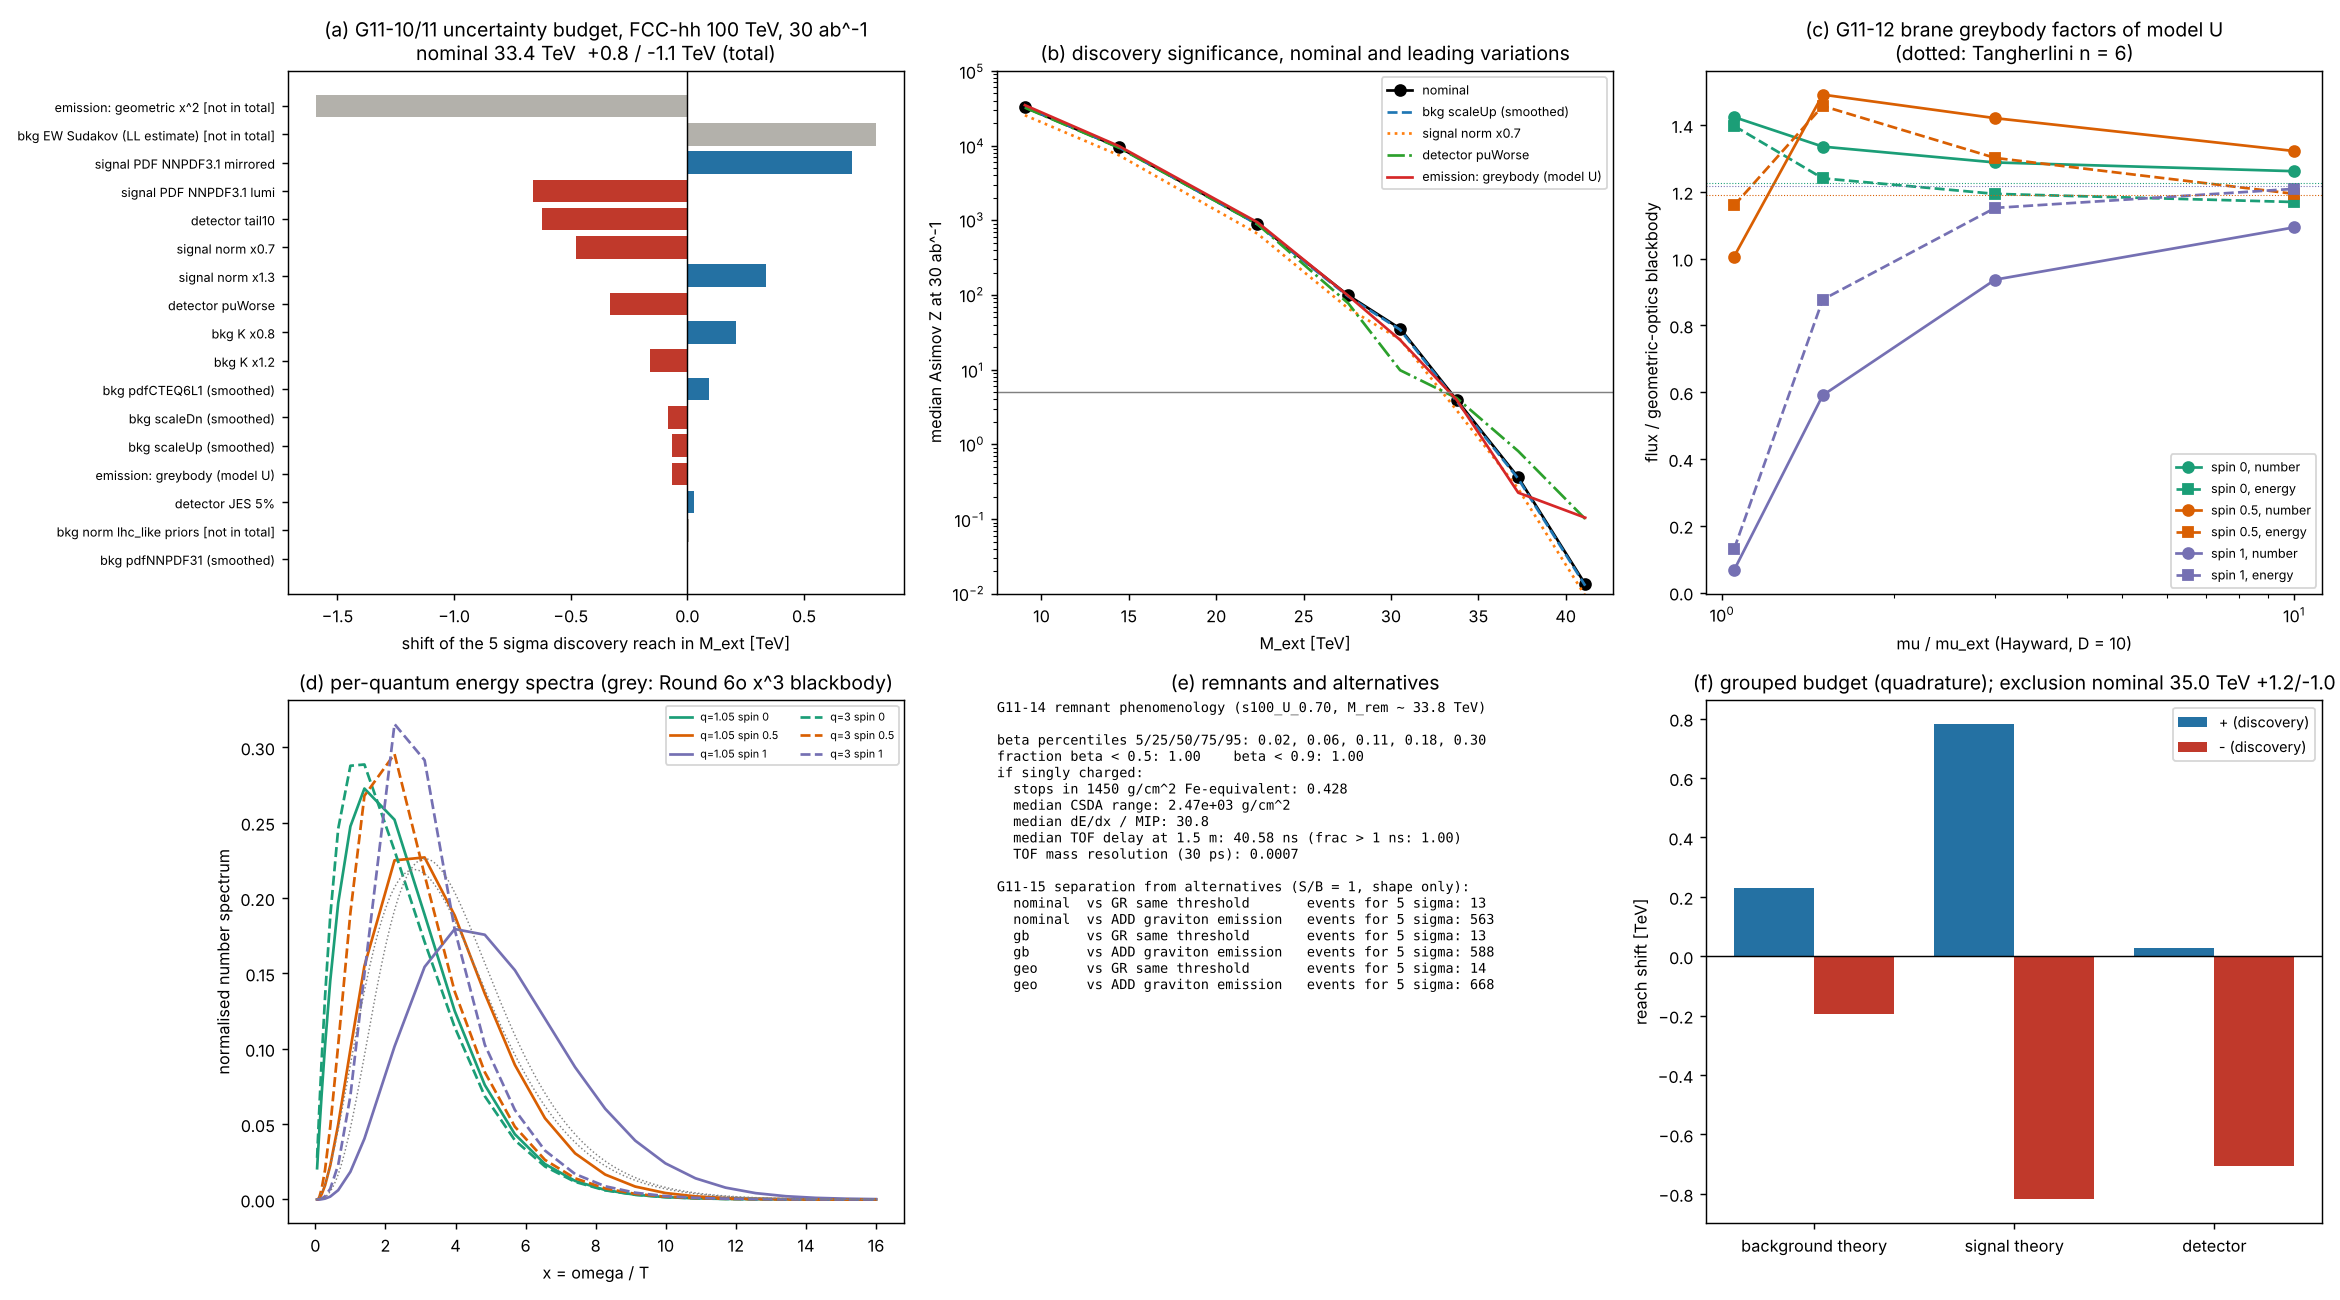
\includegraphics[width=\textwidth]{round11_collider.png}
\caption{(a) Budget; (b) significance versus $M_{\rm ext}$ with leading variations; (c,d) greybody factors and spectra; (e) remnants and
alternatives; (f) grouped budget.}\end{figure}

\section{Remnants and alternatives}
Remnants are slow ($\beta$ median $0.11$, all below $0.5$). Neutral remnants are pure missing energy (the default after colour
discharge). Charged remnants would be highly ionising ($\sim31\times$ MIP), arrive $\sim41$\,ns late at 1.5\,m, and $\sim40\%$ would stop
in an assumed $1450\,\mathrm{g\,cm^{-2}}$ of calorimeter (uncertain by a factor $\sim2$ at low $\beta\gamma$). The exact likelihood-ratio
separation at $S/B=1$ requires 13 events against a GR hole with the same threshold, 560--670 against ADD graviton emission and 240--370
against dark-matter mediators, robust under the emission-model variations.

\section{Current data}
The 13\,TeV ATLAS monojet likelihood excludes $M_{\rm ext}<3.5$--$4.2$\,TeV (head-on trapping) or $<6.6$--$7.2$\,TeV (full trapping)
for $n=4$--$6$, $M_D=2$--$4$\,TeV; multi-object black-hole searches accept $\le0.4\%$ of model-U events and do not constrain it.
A run on CMS Open Data is prepared but could not be executed here (network access to the open-data portal was not available).

\section*{Reproducibility}
Configuration: \texttt{ROUND11/collider/analysis\_config.json}; software versions, PDF hashes, process cards, seeds and sample hashes:
\texttt{DATA/round11\_manifest.json}; scripts \texttt{round10a.py}, \texttt{round11a.py}, \texttt{round11\_greybody.py},
\texttt{round11b.py}.

\section*{References}\small
Bueno, Cano, Hennigar, arXiv:2403.04827. Dimopoulos, Landsberg, PRL 87, 161602 (2001). Giddings, Thomas, PRD 65, 056010 (2002).
Yoshino, Nambu, PRD 67, 024009 (2003). Kanti, March-Russell, hep-ph/0203223, hep-ph/0212199. Bierlich et al., SciPost Phys.\ Codebases 8
(2022). NNPDF, Nucl.\ Phys.\ B 867, 244 (2013). ATLAS, PRD 103, 112006 (2021). CMS, PRD 97, 092005 (2018). Cowan, Cranmer, Gross, Vitells,
EPJC 71, 1554 (2011). Lindert et al., EPJC 77, 829 (2017). Becher, Garcia i Tormo, arXiv:1305.4202. K\"uhn, Kulesza, Pozzorini, Schulze,
hep-ph/0507178. FCC Collaboration, EPJ ST 228, 755 (2019).
\end{document}
